\documentclass{beamer}

\usepackage{verbatim}
%\usepackage{verbatimbox}
\usepackage{parskip}
\usepackage{geometry}
\usepackage[colorlinks=true]{hyperref}
%\usepackage{csquotes}
%\usepackage{framed}

\title{Multivariate Analysis using SPSS \\ \small{\underline{Bivariate \& Multivariate Analysis - Correlation \& Regression}}}
\author{Dr. M. Kamakshaiah \\ Assistant Professor - Business Analytics, \\ GSIB - GITAM \tiny{(Deemed to be University)} \\ \small{kamakshaiah.musunuru@gitam.edu} \\ \vspace{2cm} 
\includegraphics[height=1cm, width=1cm]{gitam_logo} 
\includegraphics[height=1cm, width=1cm]{gsib_logo}}



\date{}

\begin{document}
\titlepage 
\tableofcontents

\section{Bivariate Correlation}

\begin{frame}{Correlation - Relationship}
\centering 
In statistics, dependence or association is any statistical relationship, whether \underline{causal} or not, between two random variables or bivariate data. \emph{Correlation} is any of a broad class of statistical relationships involving dependence, though in common usage it most often refers to how close two variables are to having a \underline{linear relationship} with each other.
	
\end{frame}

\begin{frame}
	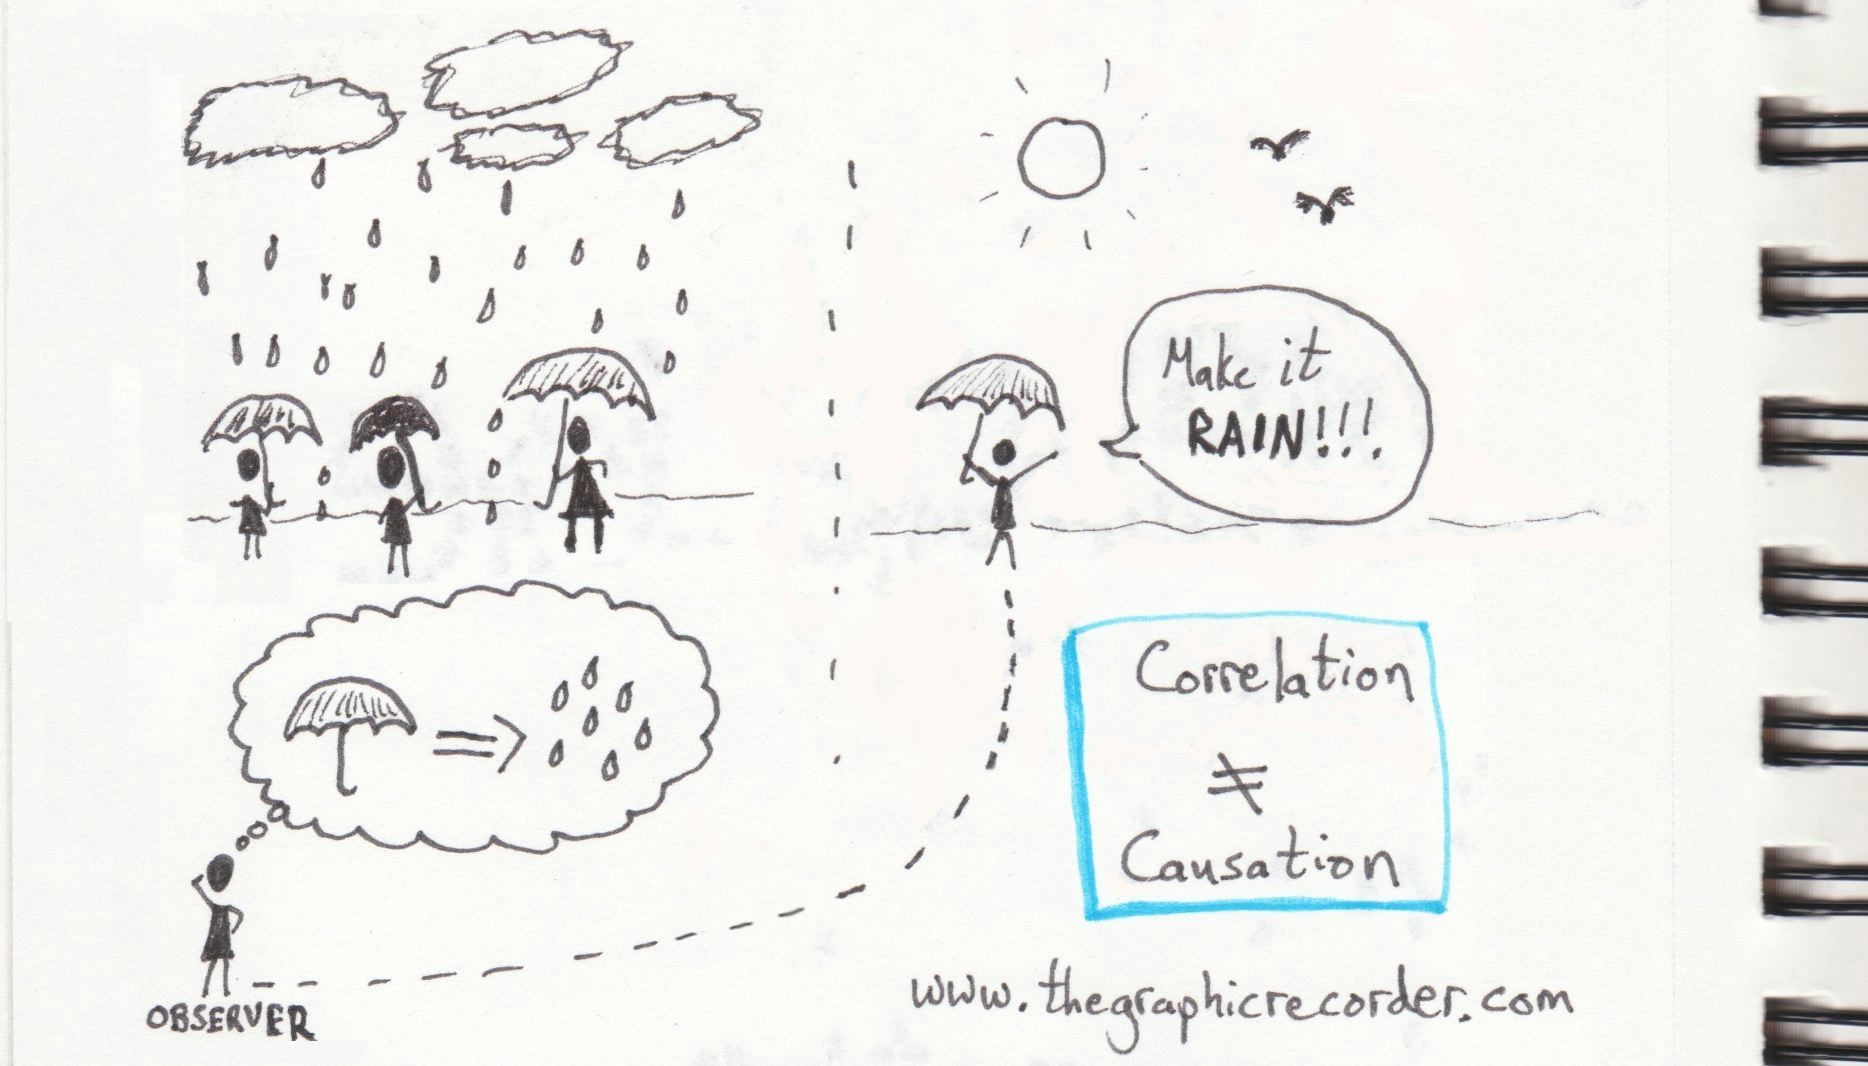
\includegraphics[height=7cm, width=10cm]{cor_cause}
\end{frame}

\begin{frame}

\includegraphics[height=7cm, width=10cm]{cor_cause_1}	
\end{frame}

\begin{frame}{Patterns}
\centering 
	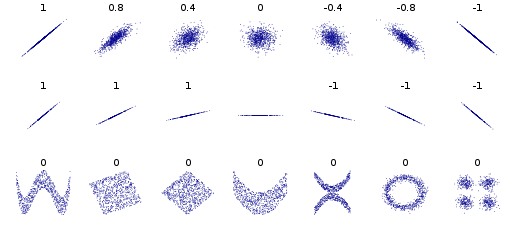
\includegraphics[height=5cm, width=9cm]{cor_ex}\\ 
	\underline{Exercise}: Use Excel spreadsheet to make visuals
\end{frame}

\subsection{Correlation coefficient}

\begin{frame}{Correlation coefficient}
	\centering 
	A correlation \emph{coefficient} is a numerical measure of some type of correlation, meaning a statistical relationship between two variables. \\ 
	
	The variables may be two columns of a given data set of observations, often called a sample, or two \emph{\underline{components}} of a multivariate random variable with a known distribution.
\end{frame}

\begin{frame}{Correl. Coef. - Interpretations}

\begin{enumerate}
	\item They all assume values in the range from -1 to +1, where +1 indicates the strongest possible agreement and -1 the strongest possible disagreement.
	\item The \emph{Pearson product-moment correlation coefficient}, also known as \emph{Pearson's r}, is a measure of the strength and direction of the linear relationship between two variables. 
	\begin{itemize}
	\item $-0.3 <= r <= 0.3$ (Weak)
	\item $ \pm 0.5 <= r <= \pm 0.7$ (Moderate)
	\item $ r > \pm 0.7 $ (Strong)
	\end{itemize} \footnote{Dr. Smith, Interpreting Correlation Coefficents, Available at \url{https://campus.fsu.edu}} \footnote{D. J. Rumsey, How to Interpret a Correlation Coefficient \emph{r}. Retrieved from \url{http://www.dummies.com/education}}
	
\end{enumerate}
	
\end{frame}

\subsubsection{Cos $\theta$}

\begin{frame}{Cos Function}
	\begin{center}
$\cos \theta ={\frac {\mathbf {x} \cdot \mathbf {y} }{\left\|\mathbf {x} \right\|\left\|\mathbf {y} \right\|}}$
	\end{center}
	\vfill 
	Note: SPSS can't help you!
\end{frame}

\subsubsection{Karl Pearson's r}

\begin{frame}{Karl Pearson's \emph{r}}
	Defined as the \underline{covariance} of the variables divided by the product of their \underline{standard deviations}. \\ \vspace{1cm}
	For Population - 
	\begin{center}
	$ \rho _{X,Y}={\frac {\operatorname {cov} (X,Y)}{\sigma _{X}\sigma _{Y}}} $	
	\end{center}
	
		\vspace{1cm}
	For Sample - 
	
\begin{center}
$r={\frac {\sum _{i=1}^{n}(x_{i}-{\bar {x}})(y_{i}-{\bar {y}})}{{\sqrt {\sum _{i=1}^{n}(x_{i}-{\bar {x}})^{2}}}{\sqrt {\sum _{i=1}^{n}(y_{i}-{\bar {y}})^{2}}}}}$
	
\end{center}
\end{frame}

\begin{frame}{Cos $\theta$ vs. Karl Pearson's \emph{r}}
	Excercise: make abstract or simulated data sets in Excel and try to vivisect Cos $\theta$ and Karl Pearson's \emph{r}. 
	\vfill
Note: SPSS can't help you!
\end{frame}

\subsection{Significance test}

\begin{frame}
	Pearson's correlation coefficient follows Student's t-distribution with degrees of freedom n - 2.
	
	\begin{center}
		
$t=r{\sqrt {\frac {n-2}{1-r^{2}}}} $

$r={\frac {t}{\sqrt {n-2+t^{2}}}}$
	\end{center}
\end{frame}

\subsubsection{Spearman's rank correlation}

\begin{frame}{Spearman's $\rho$}
	\centering 
	Spearman's rank correlation coefficient or Spearman's rho, often denoted by the Greek letter $\rho$  (rho) or as $r_{s}$, is a \underline{nonparametric} measure of rank correlation (statistical dependence between the rankings of two variables). 


\fbox{$r_{s}=\rho _{\operatorname {rg} _{X},\operatorname {rg} _{Y}}={\frac {\operatorname {cov} (\operatorname {rg} _{X},\operatorname {rg} _{Y})}{\sigma _{\operatorname {rg} _{X}}\sigma _{\operatorname {rg} _{Y}}}}$}

If all n ranks are distinct integers, it can be computed using the popular formula. 

\fbox{$ r_{s}={1-{\frac {6\sum d_{i}^{2}}{n(n^{2}-1)}}}$}

\end{frame}

\begin{frame}{Spearman's $\rho$} \fontsize{8} \selectfont 
	
	\begin{enumerate}
		\item The Spearman correlation between two variables is equal to the Pearson correlation between the rank values of those two variables. 
		\item Pearson's correlation assesses linear relationships, Spearman's correlation assesses monotonic relationships.
		\item If there are no repeated data values, a perfect Spearman correlation of +1 or −1 occurs. 
		\item the Spearman correlation between two variables will be high when observations have a similar rank. 
		\item Spearman's coefficient is appropriate for both continuous and discrete ordinal variables. \footnote{Lehman, Ann (2005). Jmp For Basic Univariate And Multivariate Statistics: A Step-by-step Guide. Cary, NC: SAS Press. p. 123. ISBN 1-59047-576-3.}
		\item Spearman's $\rho$  and Kendall's $\tau$  can be formulated as special cases of a more general correlation coefficient
	\end{enumerate}
	
	
\end{frame}

\subsubsection{Kendall's $\tau$}

\begin{frame}
	Kendall rank correlation coefficient, commonly referred to as Kendall's $\tau$ coefficient, is a statistic used to measure the ordinal association between two measured quantities. \\ \vspace{1cm}
	
	A tau test is a \underline{nonparametric} hypothesis test for statistical dependence based on the $\tau$ coefficient.
\end{frame}

\begin{frame}
	The Kendall $\tau$ coefficient is defined as: \vspace{1cm}
\begin{center}
$\tau ={\frac {({\text{number of concordant pairs}})-({\text{number of discordant pairs}})}{n(n-1)/2}}$ \end{center}
\vspace{1cm}

\begin{center} $\tau ={\frac {1}{n(n-1)}}\sum _{i\not =j}\operatorname {sgn}(x_{i}-x_{j})\operatorname {sgn}(y_{i}-y_{j}) $
\end{center}

\end{frame}

\subsubsection{Significance Test}
\begin{frame}{Significance Test}
	 For larger samples, it is common to use an approximation to the \underline{normal distribution}, with mean zero and variance
\vspace{1cm}
\begin{center}
$\frac {2(2n+5)}{9n(n-1)}$	
\end{center}

\end{frame}


\subsubsection{Goodman and Kruskal's $\gamma$}

\begin{frame}{Goodman and Kruskal's $\gamma$}
	Goodman and Kruskal's gamma is a measure of rank correlation, i.e., the similarity of the orderings of the data when ranked by each of the quantities. \\ \vspace{1cm}
	
	It measures the strength of association of the \underline{cross tabulated data} when both variables are measured at the ordinal level. \vspace{0.5cm}
	
	\begin{center}
		
$G={\frac  {N_{s}-N_{d}}{N_{s}+N_{d}}}$ \end{center} \vspace{0.5cm}
\begin{center} $ t\approx G{\sqrt  {{\frac  {N_{s}+N_{d}}{n(1-G^{2})}}}}$
	\end{center}
\end{frame}

\section{Canonical Correlation}

\begin{frame}{Canonical correlation}
\begin{center}
	Canonical is the statistical term for analyzing latent variables (which are not directly observed) that represent multiple variables (which are directly observed). 
\end{center}

\fontsize{8} \selectfont 
	\begin{enumerate}
		\item Canonical-correlation analysis (CCA) is a way of inferring information from cross-covariance matrices.
		\item If we have two vectors $X = (X1, ..., Xn)$ and $Y = (Y1, ..., Ym)$ of random variables, and there are correlations among the variables, then canonical-correlation analysis will find linear combinations of the $Xi$ and $Yj$ which have maximum correlation with each other.
		\item Canonical correlation analysis requires the multivariate normal and homogeneity of variance assumption.
		\item Canonical correlation analysis assumes a linear relationship between the canonical variates and each set of variables.
		\item Similar to multivariate regression, canonical correlation analysis requires a large sample size.
	\end{enumerate}
\end{frame}

\subsubsection{CCA - Methodology}

\begin{frame}{CCA - Methodology}
	\begin{center}
Let $\Sigma_{XX}=cov(X,X)$ and $\Sigma_{YY}=cov(Y,Y)$, the parameter to maximize is as follows. 

$\rho ={\frac{a^{T}\Sigma_{XY}b}{{\sqrt{a^{T} \Sigma_{XX}a}}{\sqrt{b^{T} \Sigma_{YY}b}}}}$
		
	\end{center}

Objective function: $\mathbf{a'},\mathbf{b'} ={\mbox{argmax}}_{\mathbf{a},\mathbf{b}} \operatorname{corr}(a^{T}X,b^{T}Y)$
\end{frame}	

\begin{frame}[fragile]{CCA in SPSS}
	\centering 
	There is no GUI based process in SPSS for CCA or DCA. Got to you use \underline{Syntax Window}. 
\vspace{1cm}	
	
\begin{tabular}{|p{10cm}}
	\begin{verbatim}
	manova x1 to x6
	/discrim all 
	/print = sig(eig dim). 
	execute. 
	\end{verbatim}
\end{tabular}

\end{frame}
	
\begin{frame}
	
\end{frame}























\end{document} 